\begin{table}[ht]
\centering\small
\begin{tabular}{@{}lrrrrrr@{}}
\toprule
Family & Parameter & $\bits(N)$ & Input DAG & Final DAG & Produce ms & Verify ms\\
\midrule
Fibonacci pair & 128 & 90 & 130 & 773 & 2.57 & 2.23\\
Fibonacci pair & 2,048 & 1,423 & 2,050 & 12,293 & 41.63 & 34.69\\
Binary shear pair & 128 & 129 & 131 & 264 & 1.32 & 0.99\\
Binary shear pair & 2,048 & 2,049 & 2,051 & 4,104 & 17.54 & 12.65\\
Triangular transport & 128 & 129 & 131 & 265 & 0.72 & 0.74\\
Triangular transport & 2,048 & 2,049 & 2,051 & 4,105 & 12.16 & 12.70\\
Independent blocks & 16 & 11 & 160 & 848 & 2.82 & 2.25\\
Independent blocks & 64 & 13 & 640 & 3,392 & 11.85 & 10.75\\
\bottomrule
\end{tabular}
\caption{Selected compressed benchmarks; all positive results independently
verified. Parameters are depth $n$, exponent-bit parameter $b$, transport
depth $d$, and number of blocks, respectively. $N$ is total expanded root
length, with $\bits(N)=\lfloor\log_2N\rfloor+1$. No expanded words were
materialized. Full measurements and code hashes are in the JSON.}
\label{tab:compression}
\end{table}

\begin{figure}[ht]
\centering
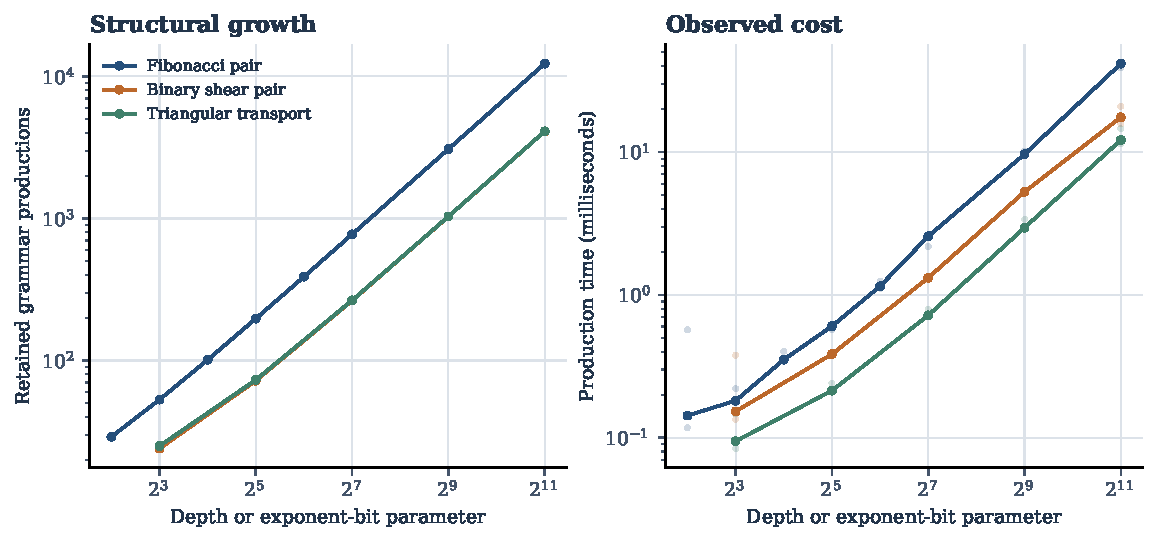
\includegraphics[width=\textwidth]{../figures/compression.pdf}
\caption{Recorded grammar sizes and elapsed production time for three
compressed families. The horizontal parameter controls exponentially large
expanded words. Straight-line growth of stored grammar sizes on these
examples illustrates the proved sharing mechanism; the finite timing curves
do not establish an asymptotic exponent.}
\label{fig:compression}
\end{figure}
